%!TEX root = ../main.tex
\chapter{Best Practices --- Testing, Documentation, Git}
\label{ch:best_practices}

\begin{intuition}
Writing code that works is one thing; writing code that is \textbf{reliable},
\textbf{readable}, and \textbf{reproducible} is another. In science, a result
must be verifiable and reproducible. This chapter presents the tools and
methods that make the difference between a throwaway script and a quality
scientific project: code style, documentation, testing, and version control.
\end{intuition}

% ----------------------------------------------------------------
\section{Code style: PEP\,8}
\index{PEP 8}\index{code style}

\begin{definition}[PEP\,8]
\textbf{PEP\,8} is the official Python style guide. It defines naming conventions,
indentation rules, and formatting guidelines to make code readable and
consistent.
\end{definition}

\begin{codeblock}[title=\textbf{Python}]
\begin{minted}{python}
# BAD STYLE
def f(x,y,z):
    A=x*y+z
    if(A>10):
        return A
    else:
        return A*2

# GOOD STYLE (PEP 8)
def compute_score(length, width, bonus):
    """Compute the score based on dimensions and bonus."""
    score = length * width + bonus
    if score > 10:
        return score
    else:
        return score * 2
\end{minted}
\end{codeblock}

\begin{bestpractice}
Essential PEP\,8 rules:
\begin{itemize}
  \item \textbf{Indentation}: 4 spaces (never tabs).
  \item \textbf{Line length}: maximum 79 characters.
  \item \textbf{Variable names}: \py{snake\_case} (e.g., \py{molar\_mass}).
  \item \textbf{Class names}: \py{CamelCase} (e.g., \py{ChargedParticle}).
  \item \textbf{Constants}: \py{UPPER\_CASE} (e.g., \py{SPEED\_OF\_LIGHT}).
  \item \textbf{Spaces around operators}: \py{x = 3 + y}, not \py{x=3+y}.
\end{itemize}
\end{bestpractice}

\begin{codeblock}[title=\textbf{Python}]
\begin{minted}{python}
# Naming conventions
BOLTZMANN_CONSTANT = 1.380649e-23    # Constant (UPPER_CASE)
temperature_kelvin = 300.0            # Variable (snake_case)

class GasMolecule:                    # Class (CamelCase)
    def __init__(self, mass, velocity):
        self.mass = mass
        self.velocity = velocity

    def kinetic_energy(self):         # Method (snake_case)
        return 0.5 * self.mass * self.velocity**2
\end{minted}
\end{codeblock}

% ----------------------------------------------------------------
\section{Docstrings and documentation}
\index{docstring}\index{documentation}

A \textbf{docstring} is a documentation string placed right after the
definition of a function, class, or module.

\begin{codeblock}[title=\textbf{Python}]
\begin{minted}{python}
def kinetic_energy(mass, velocity):
    """
    Compute the kinetic energy of an object.

    Parameters
    ----------
    mass : float
        Mass of the object in kilograms (kg).
    velocity : float
        Velocity of the object in meters per second (m/s).

    Returns
    -------
    float
        Kinetic energy in joules (J).

    Examples
    --------
    >>> kinetic_energy(2.0, 3.0)
    9.0
    """
    return 0.5 * mass * velocity**2
\end{minted}
\end{codeblock}

\begin{codeblock}[title=\textbf{Python}]
\begin{minted}{python}
# Access the documentation
help(kinetic_energy)
\end{minted}
\end{codeblock}

\begin{codeoutput}
\begin{verbatim}
Help on function kinetic_energy in module __main__:

kinetic_energy(mass, velocity)
    Compute the kinetic energy of an object.

    Parameters
    ----------
    mass : float
        Mass of the object in kilograms (kg).
    velocity : float
        Velocity of the object in meters per second (m/s).

    Returns
    -------
    float
        Kinetic energy in joules (J).
\end{verbatim}
\end{codeoutput}

\begin{remark}
The style used above is called the \textbf{NumPy style}\index{NumPy style}.
It is the standard in the scientific Python ecosystem. Other styles exist
(Google, Sphinx), but the NumPy style is the most widespread in science.
\end{remark}

% ----------------------------------------------------------------
\section{Testing with \py{assert}}
\index{assert}\index{testing}

Testing your code is like verifying an experimental measurement: you compare
the obtained result with the expected result.

\begin{codeblock}[title=\textbf{Python}]
\begin{minted}{python}
def celsius_to_kelvin(temp_c):
    """Convert a temperature from Celsius to Kelvin."""
    return temp_c + 273.15

# Simple tests with assert
assert celsius_to_kelvin(0) == 273.15, "Error: 0 deg C != 273.15 K"
assert celsius_to_kelvin(100) == 373.15, "Error: 100 deg C"
assert celsius_to_kelvin(-273.15) == 0.0, "Error: absolute zero"
print("All tests passed!")
\end{minted}
\end{codeblock}

\begin{codeoutput}
\begin{verbatim}
All tests passed!
\end{verbatim}
\end{codeoutput}

\begin{codeblock}[title=\textbf{Python}]
\begin{minted}{python}
import math

def circle_area(radius):
    """Compute the area of a circle."""
    if radius < 0:
        raise ValueError("Radius must be positive.")
    return math.pi * radius**2

# Tests
assert abs(circle_area(1) - math.pi) < 1e-10
assert abs(circle_area(0) - 0) < 1e-10
assert abs(circle_area(2) - 4 * math.pi) < 1e-10

# Test the exception
try:
    circle_area(-1)
    assert False, "Should have raised an error"
except ValueError:
    pass  # This is the expected behavior

print("All tests passed!")
\end{minted}
\end{codeblock}

\begin{codeoutput}
\begin{verbatim}
All tests passed!
\end{verbatim}
\end{codeoutput}

\begin{warning}
For floating-point numbers, \emph{never} test for exact equality.
Use a tolerance: \py{abs(obtained - expected) < 1e-10} or
\py{math.isclose(obtained, expected)}.
\end{warning}

% ----------------------------------------------------------------
\section{Version control with Git}
\index{Git}\index{version control}

\begin{definition}[Git]
\textbf{Git} is a distributed version control system. It records
the complete history of changes to a project, allowing you to go back
in time, collaborate, and work on parallel branches.
\end{definition}

\begin{center}
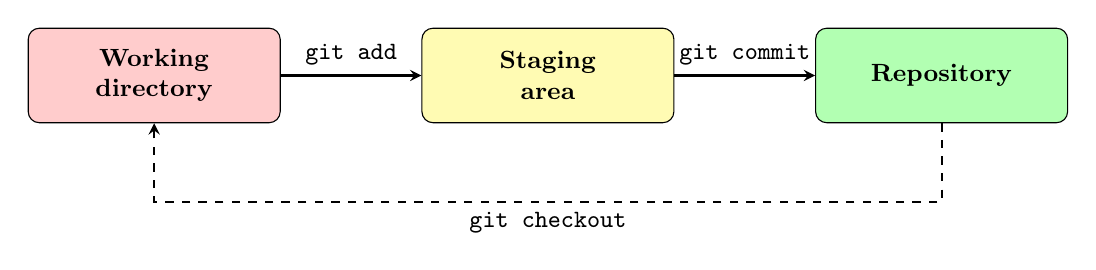
\begin{tikzpicture}[
  block/.style={draw, rounded corners, minimum width=3.2cm, minimum height=1.2cm,
                align=center, font=\small},
  arr/.style={->, thick, >=stealth},
]
  \node[block, fill=red!20] (wd) at (0,0) {\textbf{Working}\\\textbf{directory}};
  \node[block, fill=yellow!30] (stage) at (5,0) {\textbf{Staging}\\\textbf{area}};
  \node[block, fill=green!30] (repo) at (10,0) {\textbf{Repository}};

  \draw[arr] (wd.east) -- (stage.west) node[midway, above, font=\ttfamily\small] {git add};
  \draw[arr] (stage.east) -- (repo.west) node[midway, above, font=\ttfamily\small] {git commit};
  \draw[arr, dashed] (repo.south) -- ++(0,-1) -| (wd.south)
    node[pos=0.25, below, font=\ttfamily\small] {git checkout};
\end{tikzpicture}
\end{center}

\begin{codeblock}[title=\textbf{Python}]
\begin{minted}{python}
# Essential Git commands (in the terminal)
# These commands are run in a shell, not in Python

# 1. Initialize a repository
# $ git init

# 2. Check status
# $ git status

# 3. Add files
# $ git add analysis.py
# $ git add .              # Add everything

# 4. Commit
# $ git commit -m "Add initial analysis"

# 5. View history
# $ git log --oneline
\end{minted}
\end{codeblock}

\begin{example}[Typical Git session]
\begin{codeblock}[title=\textbf{Python}]
\begin{minted}{python}
# Here is a typical Git session in the terminal:
#
# $ mkdir my_project && cd my_project
# $ git init
# Initialized empty Git repository in .../my_project/.git/
#
# $ echo "print('Hello')" > main.py
# $ git add main.py
# $ git commit -m "First commit: main script"
# [master (root-commit) a1b2c3d] First commit: main script
#
# $ echo "# My Project" > README.md
# $ git add README.md
# $ git commit -m "Add README"
#
# $ git log --oneline
# b4e5f6g Add README
# a1b2c3d First commit: main script
\end{minted}
\end{codeblock}
\end{example}

% ----------------------------------------------------------------
\section{Virtual environments}
\index{venv}\index{virtual environment}

\begin{definition}[Virtual environment]
A \textbf{virtual environment} is an isolated directory containing an independent
Python installation. Each project can thus have its own dependencies without
conflicts with other projects.
\end{definition}

\begin{codeblock}[title=\textbf{Python}]
\begin{minted}{python}
# Create a virtual environment
# $ python -m venv my_env

# Activate it
# Linux/Mac:   $ source my_env/bin/activate
# Windows:     $ my_env\Scripts\activate

# Install packages
# (my_env) $ pip install numpy scipy matplotlib

# Save dependencies
# (my_env) $ pip freeze > requirements.txt

# Reproduce the environment elsewhere
# $ pip install -r requirements.txt
\end{minted}
\end{codeblock}

\begin{bestpractice}
\textbf{Always} create a virtual environment for each project.
Add the environment folder (\texttt{my\_env/}) to the
\texttt{.gitignore} file so it is not tracked by version control.
\end{bestpractice}

% ----------------------------------------------------------------
\section{Structure of a scientific project}
\index{project structure}

\begin{codeblock}[title=\textbf{Python}]
\begin{minted}{python}
# Recommended structure for a scientific project
#
# my_project/
# |-- README.md              # Project description
# |-- requirements.txt       # Dependencies
# |-- .gitignore             # Files to ignore
# |-- src/
# |   |-- __init__.py
# |   |-- analysis.py        # Analysis functions
# |   |-- visualization.py   # Plotting functions
# |-- tests/
# |   |-- test_analysis.py   # Unit tests
# |-- data/
# |   |-- measurements.csv   # Raw data
# |-- notebooks/
# |   |-- exploration.ipynb  # Jupyter notebooks
# |-- results/
#     |-- figures/            # Generated plots
\end{minted}
\end{codeblock}

\begin{codeblock}[title=\textbf{Python}]
\begin{minted}{python}
# Example .gitignore file
#
# __pycache__/
# *.pyc
# my_env/
# .ipynb_checkpoints/
# results/figures/*.png
\end{minted}
\end{codeblock}

% ----------------------------------------------------------------
\begin{errmark}{Common errors in best practices}
\begin{enumerate}
  \item \textbf{Not testing your code} --- "It seems to work" is not a
    test. Even a simple \py{assert} is better than nothing. Silent errors
    are the most dangerous in science.
  \item \textbf{Not using version control} --- Without Git, an unfortunate modification can
    destroy hours of work. Make \textbf{regular} commits with
    \textbf{descriptive} messages.
  \item \textbf{Obscure variable names} --- \py{x1}, \py{tmp}, \py{data2} convey
    nothing. Prefer \py{temperature\_kelvin}, \py{molar\_mass},
    \py{initial\_concentrations}.
  \item \textbf{Undocumented code} --- In six months, you will no longer remember
    what your function does. Add a docstring to every function.
  \item \textbf{Everything in a single file} --- Split your project into logical
    modules. A 2000-line file is difficult to maintain.
\end{enumerate}
\end{errmark}

% ----------------------------------------------------------------
\begin{projet}{Organizing a mini scientific project}
Create a complete project following best practices:
\begin{enumerate}
  \item Create the directory structure described above.
  \item Initialize a Git repository and create a \texttt{.gitignore}.
  \item In \texttt{src/analysis.py}, write three documented functions
    (for example: data loading, statistics computation, fitting).
  \item In \texttt{tests/test\_analysis.py}, write at least 5 tests with
    \py{assert}.
  \item Create a virtual environment and a \texttt{requirements.txt}.
  \item Make at least 3 Git commits with clear messages.
  \item Check your history with \texttt{git log --oneline}.
\end{enumerate}
\end{projet}

% ----------------------------------------------------------------
\section{Exercises}

\begin{exercise}[$\star$]
Fix the following code to comply with PEP\,8. Rename the variables,
add spaces, and a docstring.
\begin{minted}{python}
def f(L):
    s=0
    for i in L:
        if i>0: s+=i
    return s
\end{minted}
\end{exercise}

\begin{exercise}[$\star$]
Write a function \py{is\_prime(n)} that tests whether an integer is prime.
Add a NumPy-style docstring and at least 5 tests with \py{assert}
(including edge cases: 0, 1, 2, negative numbers).
\end{exercise}

\begin{exercise}[$\star\star$]
Create a module \texttt{physics.py} containing three documented functions:
\py{gravitational\_force(m1, m2, d)}, \py{potential\_energy(m, h)}, and
\py{pendulum\_period(L)}. Write a separate test file verifying each
function with known values.
\end{exercise}

\begin{exercise}[$\star\star$]
Initialize a Git repository in a new directory. Create a file
\texttt{calculations.py}, make a first commit. Modify the file, make a
second commit. Use \texttt{git diff HEAD\~{}1} to see the differences.
Use \texttt{git log --oneline} to display the history.
\end{exercise}

\begin{exercise}[$\star\star\star$]
Take one of your projects from previous chapters (for example the Pandas
data analysis or the SciPy fitting). Reorganize it as a structured project:
separate the code into modules, add docstrings to all functions,
write tests, create a virtual environment with \texttt{requirements.txt},
and version everything with Git (at least 5 commits).
\end{exercise}

% ----------------------------------------------------------------
\begin{keyformulas}{Chapter 11 --- Best practices: the essentials}
\begin{tabular}{@{}p{4.5cm} p{9.5cm}@{}}
\toprule
\textbf{Practice} & \textbf{Description} \\
\midrule
PEP\,8 & Official Python style: \py{snake\_case}, 4 spaces, 79 chars \\
Docstrings & Documentation embedded in the code (NumPy style) \\
\py{assert} & Verification: \py{assert obtained == expected} \\
\py{math.isclose} & Floating-point comparison with tolerance \\
\texttt{git init} & Initialize a repository \\
\texttt{git add + commit} & Record changes \\
\texttt{git log} & View history \\
\texttt{python -m venv} & Create a virtual environment \\
\texttt{pip freeze} & Save dependencies \\
\texttt{.gitignore} & Exclude files from Git tracking \\
\bottomrule
\end{tabular}
\end{keyformulas}
